\section{Virtual Kubelet}
Virtual Kubelet\cite{virtual} is an open source project by Microsoft that aims to provide a programmable kubelet API interface to developers. It was developed to run container resources on Azure Container instances without scaling the node count of running Kubernetes cluster. It has an exposed interface for extending the provided runtimes. Every virtual kubelet instance acts as an additional node and when Kubernetes calls it's methods either asyncronously or syncronously, the custom provider can answer to those queries with a runtime specific logic.

This thesis implements a new runtime provider to virtual-kubelet, that can be customised for running unikernels on different deployment environments. For example, if a node uses Xen for running unikernel images and the other one uses KVM, the provider can be customised to run respective commands without writing a new provider from scratch. 

The provider, called \textit{unikernel} is responsible for setting up the node through labels, health checking the node, and sharing node resources with the kubernetes API, so that scheduling can be done accordingly. For example the following code block is used to get resource data of the node where the virtual-kubelet is running.


% Golang Code block start
\begin{lstlisting}[language=python,caption={Get Environment data},captionpos=b]
import "runtime"
(...)
var m runtime.MemStats
runtime.ReadMemStats(&m)
cpu := strconv.Itoa(runtime.NumCPU()),
memory := strconv.Itoa(int(m.Sys/1024/1024)) + "Mi"

\end{lstlisting}
% Golang Code block end



\begin{figure}[htpb]
  \centering
  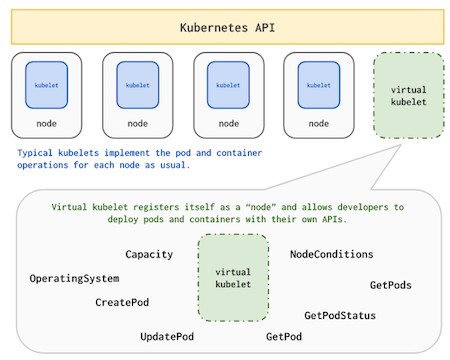
\includegraphics[width=0.8\textwidth]{figures/vk.png}
  \caption{Working principle of Virtual Kubelet \cite{virtual}} \label{fig:vk}
\end{figure}

Virtual Kubelet also opens possibilities to deploy unikernels to IoT devices through the Kubernetes API. Different virtual kubelet instances with different providers can work in parallel to deploy to target environments. This, again requires a receiver on the IoT device part. 


\subsection{Communication between cluster and device}
Kubernetes has a built-in service discovery. Deployed containers use hostnames instead of IPs to communicate between each other. Kubernetes runs a DNS server and maps those hostnames to IP addreses of individuals containers or mostly services. Unikernel deployments should also have the same functionality to work flawlessly with the rest of the kubernetes cluster. 

\subsection{Communication between kubernetes and hypervisor}
Kubernetes has a single endpoint for all the communication between the user and the cluster. This single endpoint should be aware of unikernel deployments so that it can schedule them accordingly. Kubernetes provides different ways to achieve this extensibility. First, it allows developers to create custom resource definitions such that they can be used together with other kubernetes resources. Second, kubernetes allow for deployment for different scheduler that can operate on specificly-tagged deployments. 
